\chapter*{\textbf{Эксперимент №3: Исследование эффективности программной предвыборки}}
\addcontentsline{toc}{chapter}{Эксперимент №3: Исследование эффективности программной предвыборки}

\subsection*{\textbf{Цель эксперимента}}
Выявление способов ускорения вычислений благодаря применению предвыборки данных. 

\subsection*{\textbf{Исходные данные}}
Степень ассоциативности и размер TLB данных.

\subsection*{\textbf{Описание проблемы}}
Обработка больших массивов информации сопряжена с открытием большого количества физических страниц памяти. При первом обращении к странице памяти наблюдается увеличенное время доступа к данным. Это связано с необходимостью преобразования логического адреса в физический адрес памяти, а также c открытием страницы динамической памяти и сохранения данных в кэш-памяти.

Преобразование выполняется на основе информации о использованных ранее страницах, содержащейся в TLB буфере процессора. Первое обращение к странице при отсутствии информации в TLB вызывает двойное обращение к оперативной памяти: сначала за информацией из таблицы страниц, а далее за востребованными данными. Предвыборка заключается в заблаговременном проведении всех указанных действий благодаря дополнительному запросу небольшого количества данных из оперативной памяти. 

\subsection*{\textbf{Результаты эксперимента}}
На рисунке \ref{img:experiment_3} представлен график, полученный в результате эксперимента с исходными параметрами:
\begin{itemize}
	\item Шаг увеличения расстояния между читаемыми данными
	(Б) = 512;
	\item Размер массива (К) = 128.
\end{itemize}

\begin{figure}[H]
	\centering{
		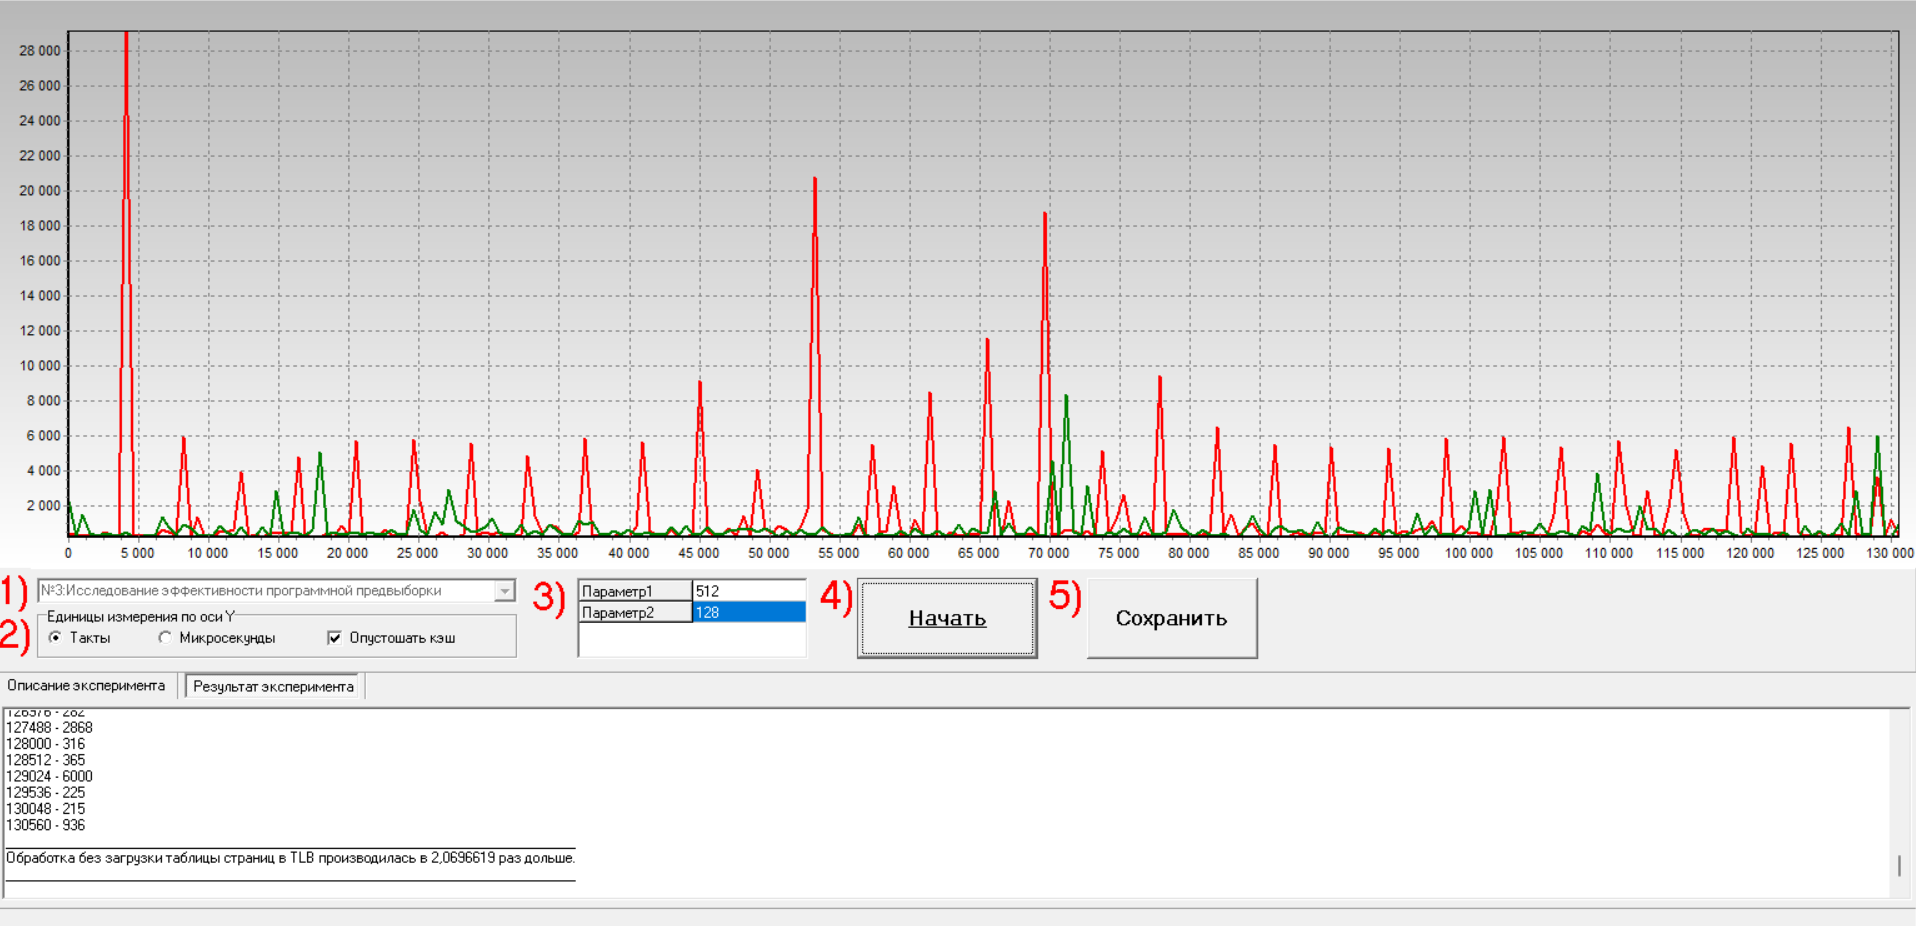
\includegraphics[scale=0.4]{images/experiment_3_1}
		\caption{Эксперимент №3}
		\label{img:experiment_3}
	}
\end{figure}

Результат сравнения времени (как вывод программы) представлен на рисунке \ref{img:experiment_3}. Как видно на рисунке, обработка без загрузки таблицы страниц в TLB производилась в 2,06 раз дольше.

Красный график - чтение страниц последовательно из оперативной памяти. Зеленый график - чтение страниц, используя дополнительный цикл предвыборки, обеспечивающий своевременную загрузку информации в TLB данных.

Сокращение времени работы алгоритма, который использует предвыборку, происходит в том случае, когда информация о востребованных страницах помещается в TLB. 

Пики на красном графике происходят из-за того, что процессу необходимо преобразовать физический адрес в логический.

\subsection*{Вывод}
Используя предвыборку можно ускорить время работы программы почти в 2 раза за счет заблаговременной загрузки страниц в память.